% Automatically generated by build/make_report.py --tex  (edit the Python script, not this file)
% Compile with:  xelatex Report.tex   (or pdflatex / lualatex; run it twice)
\documentclass[10pt,a4paper]{article}
\usepackage[T1]{fontenc}
\usepackage[utf8]{inputenc}
\usepackage{lmodern}
\usepackage[a4paper,left=2.0cm,right=2.0cm,top=1.9cm,bottom=2.3cm]{geometry}
\usepackage{graphicx,array,colortbl,xcolor,microtype,fancyhdr,titlesec,enumitem,textcomp}
\usepackage[hidelinks]{hyperref}
\definecolor{ink}{HTML}{0B0B0B}
\definecolor{grey}{HTML}{52514E}
\definecolor{blue}{HTML}{1C5CAB}
\definecolor{hdr}{HTML}{1C5CAB}
\definecolor{hl}{HTML}{FCE9E1}
\definecolor{rule}{HTML}{E1E0D9}
\color{ink}
\setlength{\parindent}{0pt}
\setlength{\parskip}{4.5pt}
\linespread{1.04}
\setlength{\tabcolsep}{3pt}
\sloppy
\titleformat{\section}{\fontsize{13.5}{16}\bfseries\color{blue}}{}{0pt}{}
\titleformat{\subsection}{\fontsize{11}{13}\bfseries\color{ink}}{}{0pt}{}
\titlespacing*{\section}{0pt}{10pt}{3pt}
\titlespacing*{\subsection}{0pt}{7pt}{2pt}
\pagestyle{fancy}
\fancyhf{}
\renewcommand{\headrulewidth}{0pt}
\fancyfoot[C]{\footnotesize\color{grey}IS3240 Group Project -- Hong Kong rental price benchmark \quad|\quad Page \thepage}
\begin{document}

{\fontsize{20}{24.0}\selectfont \color{blue} \raggedright \textbf{What should a Hong Kong host charge?}\par}\vspace{-4.5pt}
{\fontsize{13}{15.6}\selectfont \color{ink} \raggedright A machine-learning pricing benchmark for short- and mid-term rentals\par}\vspace{-2.5pt}
{\fontsize{8.5}{10.2}\selectfont \color{grey} \raggedright IS3240 Advanced Business Programming in Python \textperiodcentered{} Group Project report \textperiodcentered{} \textbf{Group:} [Group name] \textperiodcentered{} \textbf{Members:} [names and SIDs] \textperiodcentered{} 18 November 2026\par}\vspace{1.5pt}
\section*{Executive summary}
{\textbf{The decision.} Hong Kong hosts and property managers must set a nightly price for every listing, but the market is really two markets: 43\% of listings require a stay of 28+ nights (monthly rentals), which are priced at a fraction of a tourist night. Most operators price by eyeballing a few comparable listings. We ask whether machine learning in Python can give them a better, \textit{explainable} price benchmark, and whether following it matters commercially.\par}
{\textbf{What we did.} We combined Inside Airbnb's Hong Kong listings (snapshot of 25 Sep 2026) and 122,715 guest reviews with MTR-station locations collected from OpenStreetMap. After documented cleaning we modelled 5,555 bookable listings from 1,175 hosts. We compared a comparable-listings baseline with linear regression, random forest and gradient boosting, validating on \textbf{hosts the model had never seen}.\par}
{\raggedright \textbf{What we found.}\par}\vspace{-3.5pt}\nopagebreak[4]
\begin{itemize}[leftmargin=0.55cm,itemsep=2pt,topsep=2pt,parsep=0pt]
\item \textbf{The benchmark works, with honest limits.} On unseen hosts, the gradient boosting model cuts the pricing error by \textbf{27\%} versus comparable-listings pricing (MAE 267 vs 366 HKD; 95\% CI 20\%--33\%); the typical miss is 20\% and 51\% of listings are predicted within $\pm$20\%. A price band that is nominally 80\% covers 84\% of unseen listings.
\item \textbf{Stay length is the master variable.} A monthly-stay policy goes with a median nightly price 42\%--67\% lower (depending on room type), and scrambling the stay-policy information is the most damaging test for the model (+21 points of typical error); weekend check-ins carry roughly 11\%--14\% higher predicted prices on short stays.
\item \textbf{Transit access is not what the market prices.} With a median listing only 290 m from an MTR station, scrambling transit and centrality raises the typical error by only 0.4 points. Property, stay policy and the amenities that mark the listing type matter far more.
\item \textbf{The commercial risk sits above the benchmark.} 49\% of listings are in line, 24\% are $\geq$25\% above and 28\% $\geq$20\% below. Each +10\% above benchmark is associated with about 6\%--7\% fewer reviews (a demand proxy): the priciest quintile (about 69\% above) gets 4.9 reviews a year against 9.7 for listings in line, while discounts of 22\%--40\% below benchmark bring only 10.1 and 10.6 -- little extra demand for a lot of foregone price.
\end{itemize}
\vspace{3pt}{\textbf{What we recommend.} Price with a \textit{benchmark band} rather than a single number, separate weekday, weekend and monthly prices, treat the price-gap audit as a trigger for review (especially listings far above benchmark), and use the segment map to choose where to compete. The notebook ships the benchmark as a reusable function that also explains \textit{why} a price is what it is in plain language (SHAP values worded by a language model, with a number check), plus a listing-level price audit file.\par}
\section*{1. Business problem and motivation}
{Short-term rental platforms have turned thousands of Hong Kong flats into accommodation, from spare rooms to whole flats run by professional operators (hosts with five or more listings own 73\% of all listings; the largest runs 344). Every operator faces the same recurring question: \textit{what nightly price should this listing carry?} Too high and the listing sits empty; too low and revenue is given away on every night booked. The question is harder here than in most cities for two reasons. First, \textbf{the market is two markets}: Hong Kong requires a licence for accommodation let for fewer than 28 consecutive days (Hotel and Guesthouse Accommodation Ordinance, Cap. 349), and 43\% of listings set a minimum stay of 28 nights or more. Second, price depends on many interacting attributes (district, size, transit, amenities, host type), and operators typically fall back on looking at a handful of 'comparable' listings.\par}
{\textbf{Our objective} is a \textit{pricing benchmark} that (i) predicts a fair asking price and a plausible band from information available \textbf{before the first guest arrives}, (ii) explains what drives price and by how much, (iii) flags listings priced far from the benchmark, and (iv) tests whether being priced above or below it is associated with demand. The users are \textbf{hosts and property managers} (set and review prices, decide on upgrades), \textbf{investors} (choose segments and districts) and, indirectly, \textbf{platforms and policy makers} (size of the monthly segment). Machine learning is appropriate because the relationship between attributes and price is non-linear and interacting, the data are rich (91 columns, 122k reviews), and the benefit of better pricing recurs with every listing and every night. The report follows the story-telling logic of the course -- \textit{why the question is valuable, which factors matter and why, how they are computed, why the models are suitable, and how well they perform} -- and then turns the result into decisions.\par}
\section*{2. Data and preparation}
{\textbf{Sources.} (1) Inside Airbnb \textit{detailed listings} for Hong Kong: 6,614 listings $\times$ 91 columns, scraped 25 Sep 2026. (2) Inside Airbnb \textit{reviews}: 122,715 comments on 3,731 listings (2011--2026). (3) \textbf{98 Hong Kong MTR stations} that we collected from OpenStreetMap through the Overpass API (a web-data-collection step using \texttt{requests} and JSON, as in Week 4), removing Shenzhen stations and Light Rail stops and caching the result for reproducibility. The summary listings file was only used for checks (its price agrees with the detailed file for just 39\% of listings, so the files are not mixed).\par}
{\textbf{Two properties of the data shape the whole project.} First, the \texttt{price} field is the \textit{price per night of a price quote for a specific stay}; the quoted length equals the host's minimum nights for 92\% of listings. A nightly price is therefore not comparable between a 1-night and a 30-night stay, so \textbf{stay length must be a core factor}. Second, the \texttt{license} column is completely empty, so the legal status of listings cannot be analysed and we do not pretend to.\par}
{\fontsize{8.5}{10.2}\selectfont \raggedright \textbf{Table 1 -- Data preparation: every removal is counted.}\par}\vspace{-3.5pt}\nopagebreak[4]
\begin{center}{\fontsize{8}{9.6}\selectfont\arrayrulecolor{rule}\begin{tabular}{>{\raggedright\arraybackslash}p{6.08cm}>{\raggedleft\arraybackslash}p{1.78cm}>{\raggedleft\arraybackslash}p{1.48cm}>{\raggedright\arraybackslash}p{6.78cm}}
\rowcolor{hdr}\color{white}\bfseries Cleaning step & \color{white}\bfseries Listings left & \color{white}\bfseries Removed & \color{white}\bfseries Business reason\\
Listings in the detailed file & 6,614 & -- & --\\\hline
Drop listings without a price quote (mostly not bookable) & 5,603 & 1,011 & 66\% cannot be booked (availability 0); rest have no quote\\\hline
Drop listings without minimum-nights policy & 5,584 & 19 & Cannot be assigned to a stay regime\\\hline
Drop implausible prices (< 50 or > 7,534 HKD) & 5,555 & 29 & Data errors (e.g. a 0.73 HKD tent) and the top 0.5\% (> 7,534 HKD): outside typical host pricing\\\hline
\end{tabular}}\end{center}
{The modelling sample therefore has \textbf{5,555 listings (84\% of the file)} with a median price of 471 HKD per night. The price is strongly right-skewed (skewness 3.1), so we model \textbf{log-price}, which makes errors percentages -- the way a host thinks (``I am 20\% above market'').\par}
\section*{3. Understanding the market before modelling}
\begin{center}\nopagebreak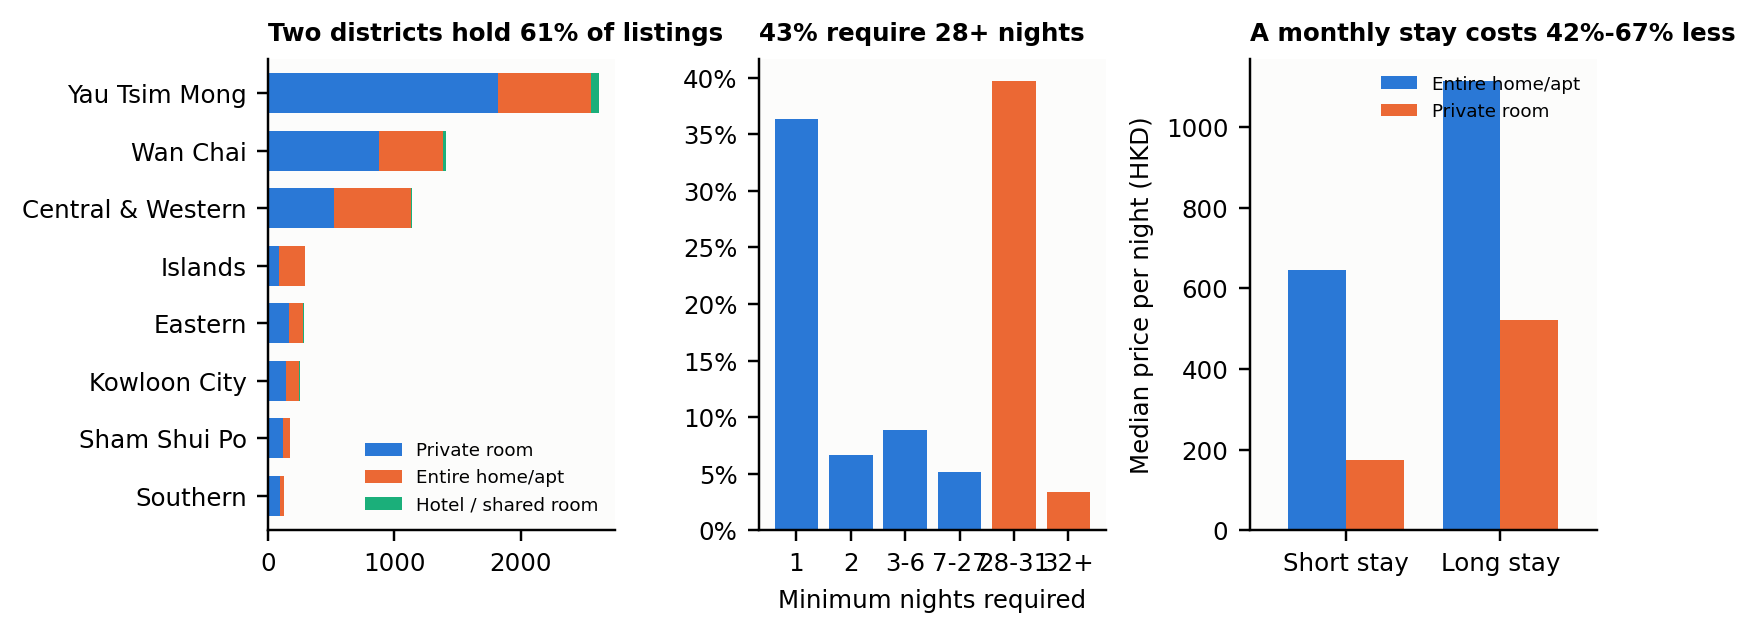
\includegraphics[width=15.2cm]{outputs/figures/fig1_market_overview.png}\end{center}\vspace{-6pt}\nopagebreak[4]
{\fontsize{8.5}{10.2}\selectfont \color{grey} \raggedright \textbf{Figure 1 -- The market at a glance.} (a, b) all 6,614 listings; (c) the modelling sample. Source: Inside Airbnb, 25 Sep 2026; authors' analysis.\par}\vspace{4pt}
{Figure 1 gives three facts that structure the analysis. \textbf{Supply is concentrated}: Yau Tsim Mong and Wan Chai hold 61\% of listings, and private rooms are 61\% of all listings. \textbf{Monthly rentals are a market of their own}: 43\% of listings require 28+ nights, and their nightly price is 67\% lower for private rooms and 42\% lower for whole homes. A fourth fact comes from the geography we added (section 2): \textbf{raw geography is a weak signal}: because supply is built where transit is, half of all listings are within 300 m of an MTR station, and median prices relative to similar listings are flat across distance bands (about -1\% within 250 m versus 6\% at 1--2 km). Premiums appear mainly outside the urban core. This warns that location effects are entangled with the type of property offered, which is why a multivariate model is needed.\par}
\begin{center}\nopagebreak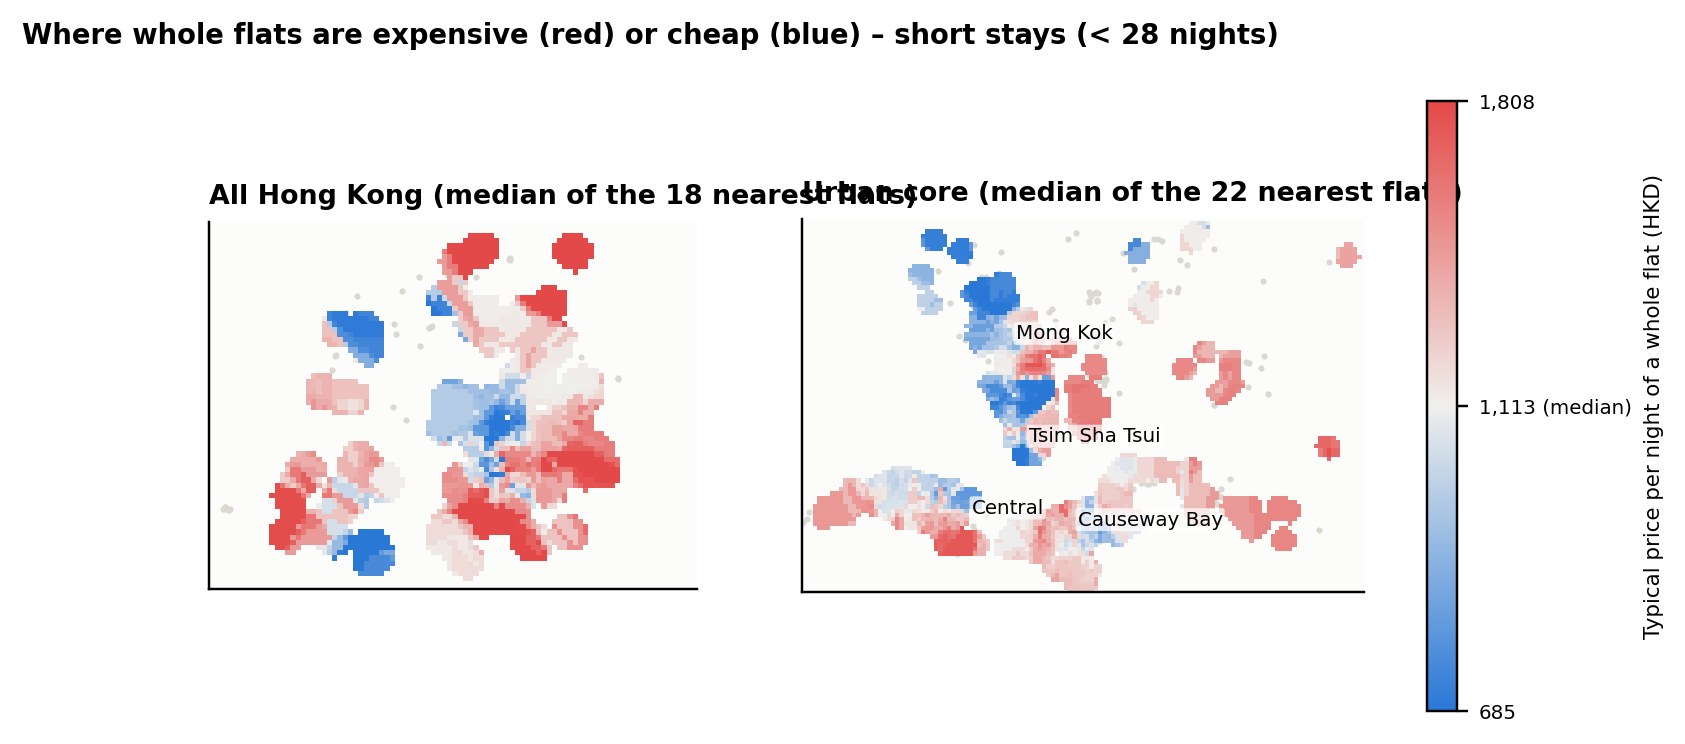
\includegraphics[width=15.2cm]{outputs/figures/fig2b_price_map.png}\end{center}\vspace{-6pt}\nopagebreak[4]
{\fontsize{8.5}{10.2}\selectfont \color{grey} \raggedright \textbf{Figure 2 -- Where whole flats are expensive (red) or cheap (blue) for short stays.} Each point shows the median relative price of the 18--22 nearest whole flats on a scale centred on the Hong Kong median (1,113 HKD per night); blank = no flats nearby. Monthly stays: Figure A1.\par}\vspace{4pt}
{The price map answers the first question any host or investor asks. For \textbf{short stays}, a whole flat has a median asking price of 1,113 HKD per night, and the cheap and expensive zones are not where one might expect: central Kowloon (Mong Kok -- Jordan -- Tsim Sha Tsui) shows the cheapest zones of the urban core, while the south and east of Hong Kong Island and parts of Lantau and the New Territories are the most expensive. Among districts with at least 30 whole flats, Eastern is the dearest (median 1,294 HKD) and Yau Tsim Mong the cheapest (957 HKD, 26\% lower). The map shows \textit{levels}, not causes: a red zone can simply hold larger flats, which is why the models below control for size, type and stay before attributing a premium to location.\par}
\begin{center}\nopagebreak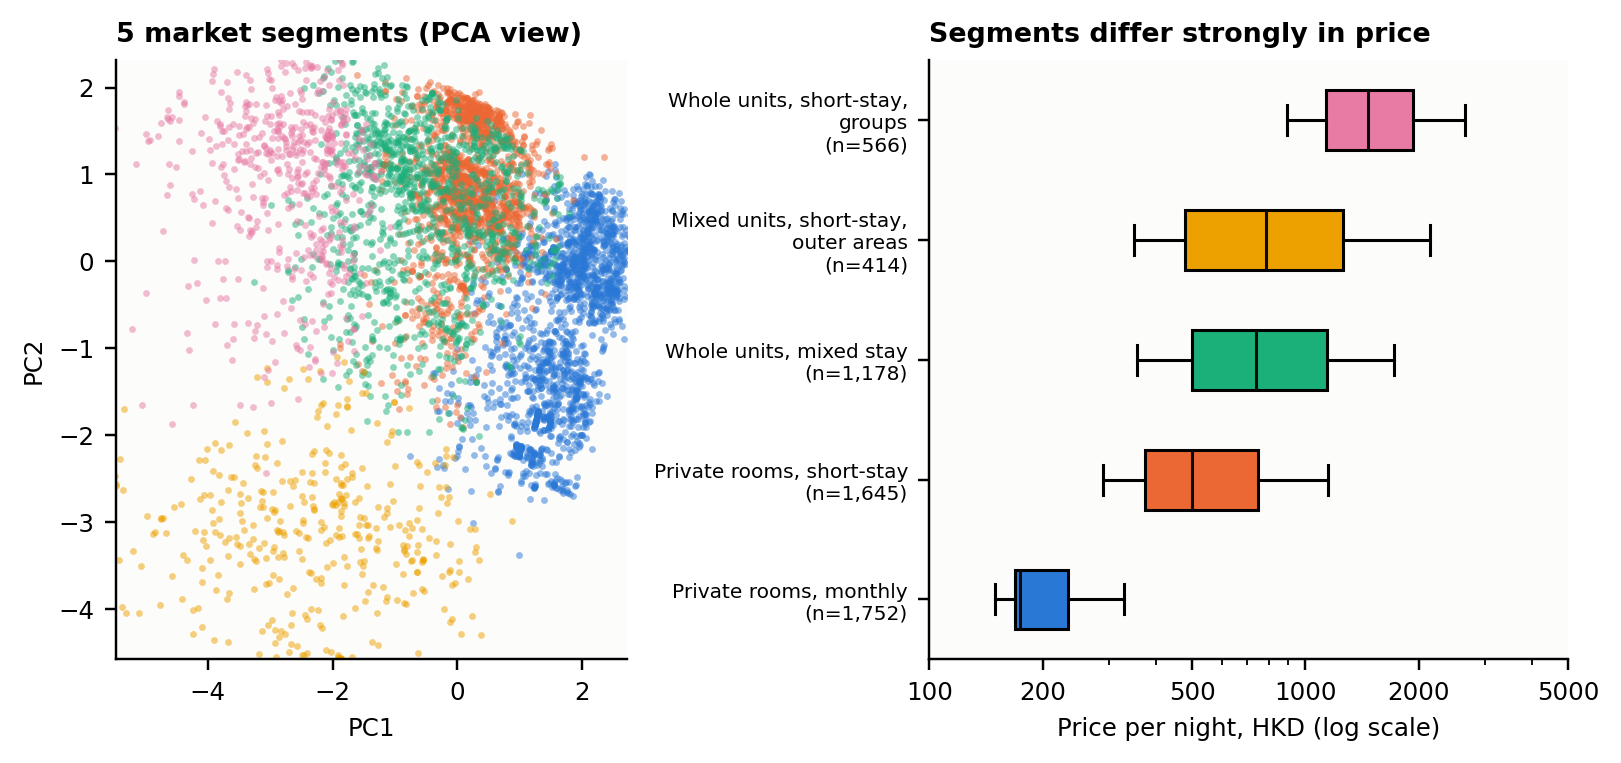
\includegraphics[width=15.2cm]{outputs/figures/fig3_segments.png}\end{center}\vspace{-6pt}\nopagebreak[4]
{\fontsize{8.5}{10.2}\selectfont \color{grey} \raggedright \textbf{Figure 3 -- Five market segments found with KMeans (k chosen by silhouette, every segment $\geq$ 3\% of listings; price was not an input) and their price distributions.}\par}\vspace{4pt}
{\fontsize{8.5}{10.2}\selectfont \raggedright \textbf{Table 2 -- Market segments.}\par}\vspace{-3.5pt}\nopagebreak[4]
\begin{center}{\fontsize{8}{9.6}\selectfont\arrayrulecolor{rule}\begin{tabular}{>{\raggedright\arraybackslash}p{5.98cm}>{\raggedleft\arraybackslash}p{1.28cm}>{\raggedleft\arraybackslash}p{2.58cm}>{\raggedleft\arraybackslash}p{1.98cm}>{\raggedleft\arraybackslash}p{1.98cm}>{\raggedleft\arraybackslash}p{1.88cm}}
\rowcolor{hdr}\color{white}\bfseries Segment (KMeans) & \color{white}\bfseries Share & \color{white}\bfseries Median price (HKD) & \color{white}\bfseries Monthly stays & \color{white}\bfseries Median guests & \color{white}\bfseries Pro hosts (5+)\\
Private rooms, monthly & 32\% & 174 & 97\% & 1 & 98\%\\\hline
Private rooms, short-stay & 30\% & 500 & 4\% & 2 & 83\%\\\hline
Whole units, mixed stay & 21\% & 739 & 37\% & 2 & 61\%\\\hline
Whole units, short-stay, groups & 10\% & 1,470 & 16\% & 7 & 55\%\\\hline
Mixed units, short-stay, outer areas & 7\% & 787 & 16\% & 2 & 25\%\\\hline
\end{tabular}}\end{center}
{The segmentation reveals an industrial structure hidden behind the word 'Airbnb': the largest segment (\textbf{private rooms, monthly, 32\% of listings}) consists of single-guest rooms rented by the month at a median of 174 HKD per night, and 98\% of them are run by professional hosts -- a co-living-style business, not tourism. A host should benchmark against their own segment, and an investor should choose a segment before choosing a district.\par}
\section*{4. Method: from useful factors to a benchmark you can trust}
{\textbf{Factors and why they should matter.} We follow \textit{hedonic pricing theory} (Rosen, 1974): a listing is a bundle of attributes and its price reflects what guests pay for each. We built 56 launch-time factors in 7 families, each with a business rationale (Table 3) and following the feature-construction logic of Xu et al. (2022); all are computed in Python from the raw files (regular expressions for bathrooms, JSON parsing and flags for amenities, haversine distances to MTR stations and hubs). A separate set of ratings and review-activity factors exists only after a listing has guests; it is excluded from the benchmark for new listings and used in a second model for existing ones. We deliberately excluded the quote's lead time because it partly reflects demand (leakage).\par}
{\fontsize{8.5}{10.2}\selectfont \raggedright \textbf{Table 3 -- Launch-time factor families.}\par}\vspace{-3.5pt}\nopagebreak[4]
\begin{center}{\fontsize{8}{9.6}\selectfont\arrayrulecolor{rule}\begin{tabular}{>{\raggedright\arraybackslash}p{3.38cm}>{\centering\arraybackslash}p{1.38cm}>{\raggedright\arraybackslash}p{11.58cm}}
\rowcolor{hdr}\color{white}\bfseries Family & \color{white}\bfseries \# factors & \color{white}\bfseries Examples and rationale\\
Property \& capacity & 8 & Room/property type, guests, bedrooms, baths, shared bathroom -- space and privacy are what guests buy\\\hline
Stay policy \& quote & 4 & 28+ night policy, quoted nights, weekend check-in -- defines the customer and the quote being priced\\\hline
Location & 4 & District, region, coordinates -- neighbourhood prestige\\\hline
Transit \& centrality & 5 & Distance to nearest MTR, stations within 1 km, distance to Central/TST -- Hong Kong is a transit city\\\hline
Local competition & 2 & Listings within 500 m / 1 km -- substitutes vs. proven tourist area\\\hline
Amenities & 31 & 30 most common amenities + count -- convenience guests trade money for\\\hline
Host profile & 2 & Professional host (5+ listings), host lives in HK -- operators price differently (richer host-history variables were tested and dropped: they did not generalise to unseen hosts)\\\hline
\end{tabular}}\end{center}
{\textbf{Models and evaluation design.} The benchmark every model must beat is \textbf{what hosts do today}: the median price of comparable listings (same district, room type and stay regime). We compare it with linear regression (transparent linear logic), random forest and gradient boosting (non-linear effects and interactions without hand-made terms). Three design decisions protect credibility: (1) \textbf{we split and cross-validate by host} (80/20 on 1,175 hosts; no host appears on both sides), because a professional host's near-identical listings would otherwise let the model memorise them and inflate accuracy; the hold-out was chosen among 50 host-level splits for composition (stay regime, price level, size) only, since one host owns 344 listings; (2) \textbf{everything learned from data uses the training part only} (the median that fills missing values, the settings of the models); (3) \textbf{models are selected by cross-validation on training data} and the 1,118-listing test set is used once. Metrics are business-first: MAE in HKD, median absolute \% error, and the share of listings predicted within $\pm$20\%.\par}
{\fontsize{8.5}{10.2}\selectfont \raggedright \textbf{Table 4 -- Key analytical decisions.}\par}\vspace{-3.5pt}\nopagebreak[4]
\begin{center}{\fontsize{8}{9.6}\selectfont\arrayrulecolor{rule}\begin{tabular}{>{\raggedright\arraybackslash}p{6.38cm}>{\raggedright\arraybackslash}p{10.18cm}}
\rowcolor{hdr}\color{white}\bfseries Decision & \color{white}\bfseries Why (business or statistical reason)\\
Treat \textbf{stay length as a core factor} and segmentation (28+ nights) & The price is a quote for a specific stay and monthly stays cost a fraction per night; it is the largest single gain in accuracy\\\hline
Drop un-priced listings; trim prices < 50 HKD or above the 99.5th percentile & A benchmark is about bookable listings; removes data errors and a few luxury outliers that dominate squared error (Table 1)\\\hline
Model \textbf{log-price} & Errors become percentages (how hosts think) and skewness falls from 3.1 to 0.4\\\hline
Split and cross-validate \textbf{by host}; choose a representative hold-out by composition only & Prevents memorising professional hosts; one host owns 344 listings, so a random split can be badly unbalanced\\\hline
Learn medians and settings on the training part only; select by CV; use the test set once & No leakage; the test result is an honest estimate\\\hline
Benchmark = \textbf{comparable-listings pricing} & The business question is 'better than what I do today?', not 'better than the global median'\\\hline
Keep only two host flags; exclude quote lead time and, for new listings, ratings and reviews & Host-history variables did not generalise to unseen hosts; lead time leaks demand; new hosts have no reviews\\\hline
Segment with KMeans \textbf{without price}; k by silhouette with segments $\geq$ 3\% of listings & Price differences between segments are findings, and every segment is big enough to act on\\\hline
Explain with permutation importance on unseen hosts; say \textit{association} & Easy to state and applies to any model; observational data, so no causal claims\\\hline
Price audit: gap = actual $\div$ benchmark $-$ 1; $\pm$25\% thresholds; demand proxy = reviews in the last 12 months, only listings with a year of history, Poisson model with controls & A new listing looks unpopular only because it is new; reviews are a count; controls compare like with like (a proxy, so we claim association only)\\\hline
Explain each price with SHAP, worded by a language model that only receives our numbers; check every number and fall back to a template & SHAP is the standard, additive explanation of a model; the language model is only a writer, so it cannot invent facts (Week 3 risks of AI text)\\\hline
Report a \textbf{band} and verify its coverage; drop the amenity-uplift ranking & Avoids false precision; amenity 'uplifts' were unstable and mostly mark listing type, so we show levers on one realistic profile instead\\\hline
\end{tabular}}\end{center}
\section*{5. Results}
\subsection*{5.1 The benchmark beats comparable-listings pricing}
\begin{center}\nopagebreak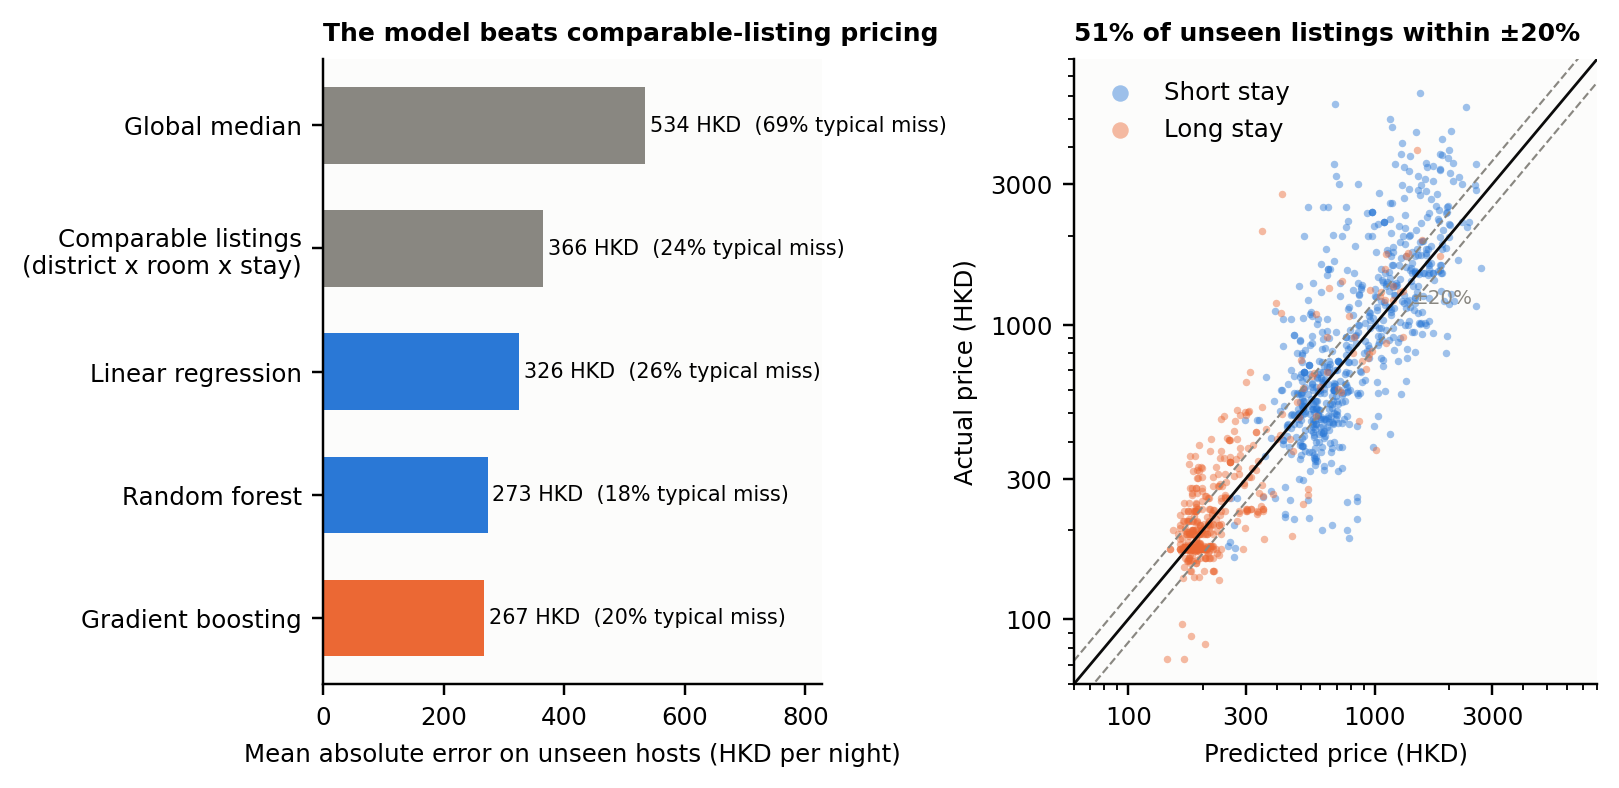
\includegraphics[width=15.2cm]{outputs/figures/fig4_model_performance.png}\end{center}\vspace{-6pt}\nopagebreak[4]
{\fontsize{8.5}{10.2}\selectfont \color{grey} \raggedright \textbf{Figure 4 -- Performance on 1,118 unseen listings (235 hosts not used in training).} Left: mean absolute error; right: predicted vs. actual price (dashed lines $\pm$20\%).\par}\vspace{4pt}
{\fontsize{8.5}{10.2}\selectfont \raggedright \textbf{Table 5 -- Model comparison on held-out hosts.} The model selected by cross-validation is highlighted.\par}\vspace{-3.5pt}\nopagebreak[4]
\begin{center}{\fontsize{8}{9.6}\selectfont\arrayrulecolor{rule}\begin{tabular}{>{\raggedright\arraybackslash}p{4.78cm}>{\raggedleft\arraybackslash}p{1.98cm}>{\raggedleft\arraybackslash}p{2.18cm}>{\raggedleft\arraybackslash}p{2.38cm}>{\raggedleft\arraybackslash}p{2.18cm}>{\raggedleft\arraybackslash}p{2.18cm}}
\rowcolor{hdr}\color{white}\bfseries Model (test set) & \color{white}\bfseries MAE (HKD) & \color{white}\bfseries RMSE (HKD) & \color{white}\bfseries Median \% error & \color{white}\bfseries Within $\pm$20\% & \color{white}\bfseries R\textsuperscript{2} (log price)\\
Global median & 534 & 890 & 68.7\% & 15\% & -0.01\\\hline
Comparable-listings baseline & 366 & 735 & 23.6\% & 46\% & 0.57\\\hline
Linear regression & 326 & 651 & 26.0\% & 40\% & 0.73\\\hline
Random forest & 273 & 582 & 18.4\% & 53\% & 0.80\\\hline
\rowcolor{hl}\bfseries Gradient boosting & \bfseries 267 & \bfseries 563 & \bfseries 19.8\% & \bfseries 51\% & \bfseries 0.80\\\hline
\end{tabular}}\end{center}
{The \textbf{gradient boosting} was selected by cross-validation on the training hosts and reduces MAE by \textbf{27\%} against comparable-listings pricing (95\% host-bootstrap CI 20\%--33\%); the other tree model is on par (MAE 273), so the conclusion does not hinge on the model family. On all 5,555 listings, host-grouped cross-validation gives the same picture (MAE 260 vs 336 HKD; typical error 23.1\%). A typical miss of about 23\% is \textit{not} a precise price -- asking prices are noisy and many hosts price by habit -- which is why the tool reports a band, and why we are explicit that this is a benchmark, not an oracle. Accuracy varies: monthly private rooms are predicted best (median error 10\%), short-stay private rooms worst (31\%), and thin districts such as Sai Kung are unreliable (few listings).\par}
\subsection*{5.2 What drives the price?}
\begin{center}\nopagebreak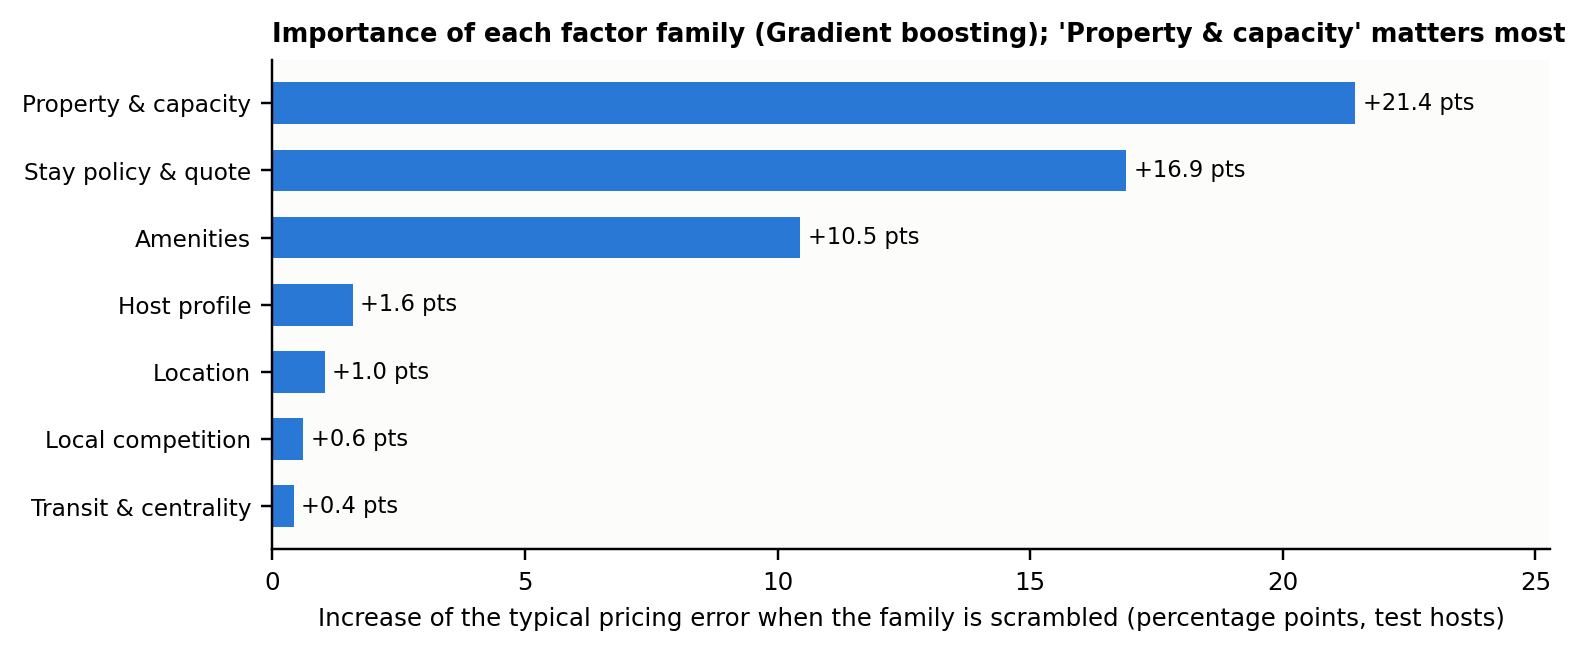
\includegraphics[width=14.6cm]{outputs/figures/fig5_importance.png}\end{center}\vspace{-6pt}\nopagebreak[4]
{\fontsize{8.5}{10.2}\selectfont \color{grey} \raggedright \textbf{Figure 5 -- Permutation importance of each factor family} (selected model, test hosts; increase of the typical pricing error, in percentage points, when the family is scrambled).\par}\vspace{4pt}
{To see which information the benchmark really uses, we scramble one family of factors at a time among the test listings and measure how much the typical error grows (permutation importance, Breiman, 2001; the typical error is 19.8\% without scrambling). \textbf{Property \& capacity} is clearly the most important family (+21.4 points), followed by Stay policy \& quote (+16.9) and Amenities (+10.5). Amenities rank high mostly because they mark the \textit{type} of listing (a flag such as a washer or a kitchen tells the model whether it is a whole flat or a room). At the other end, Location (+1.0), Local competition (+0.6) and \textbf{transit \& centrality (+0.4)} add little once the rest is known. Ratings and review activity add little for existing listings too (on test hosts with reviews the median error moves from 24\% to 22\%). \textbf{Price is mostly decided by what the listing is and how long guests stay -- not by location details, reputation or transit proximity.} This is an association: importance shows what the model uses, and correlated factors can share it.\par}
\subsection*{5.3 A price audit: who is priced away from the benchmark, and does it cost them guests?}
\begin{center}\nopagebreak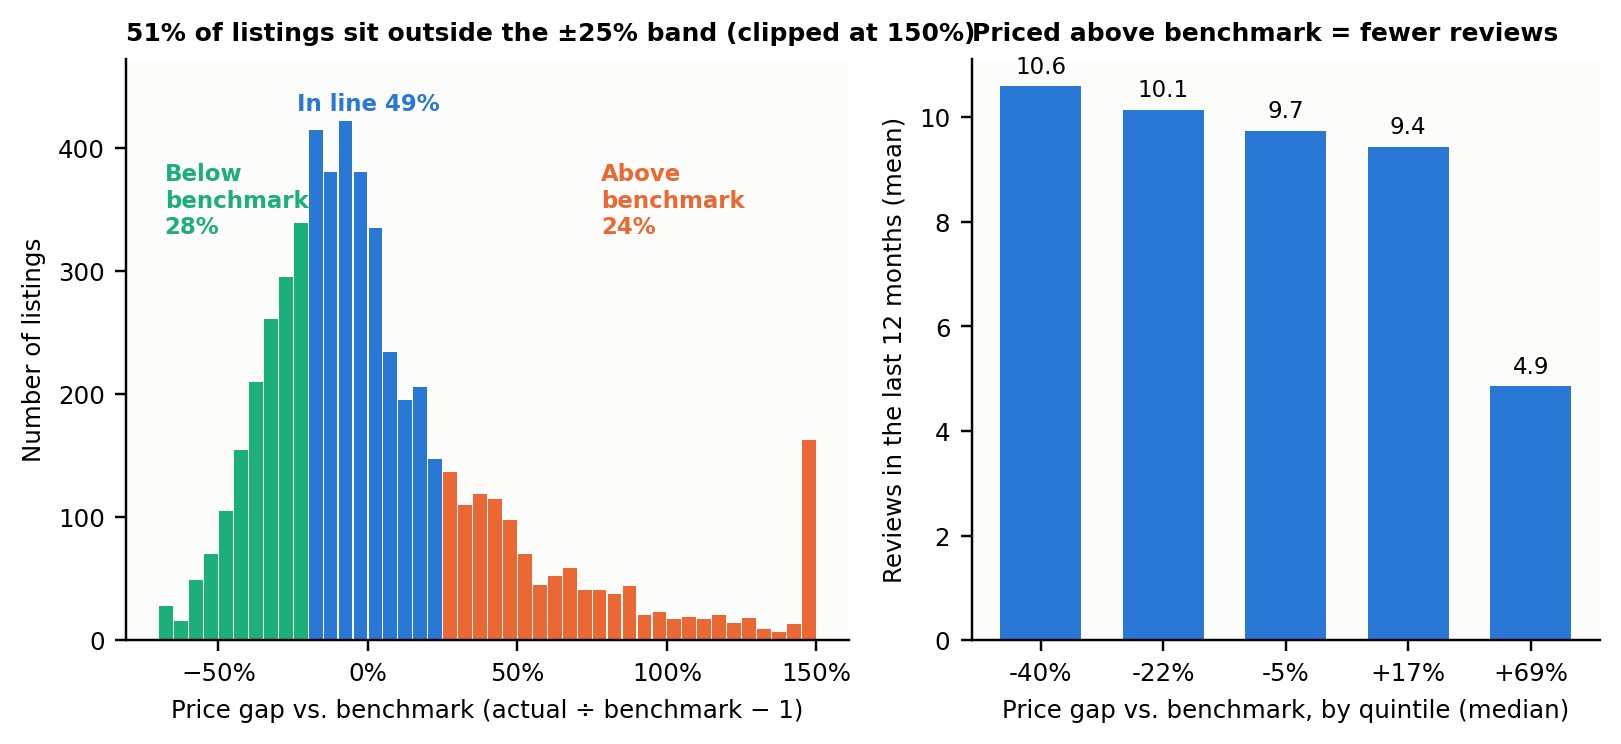
\includegraphics[width=15.2cm]{outputs/figures/fig7_price_gap_demand.png}\end{center}\vspace{-6pt}\nopagebreak[4]
{\fontsize{8.5}{10.2}\selectfont \color{grey} \raggedright \textbf{Figure 6 -- Price gap vs. out-of-fold benchmark, and reviews in the last 12 months by price-gap quintile} (2,412 listings with at least a year of history).\par}\vspace{4pt}
{Using out-of-fold predictions (each listing predicted by a model that never saw its host), \textbf{49\% of listings are in line} with their benchmark, 24\% are at least 25\% above and 28\% at least 20\% below. Reviews in the last 12 months are a demand proxy. In a Poisson model with controls for stay regime, room type, district and size, \textbf{+10\% above benchmark is associated with 5.7\% fewer reviews} (95\% CI 2.9\%--8.5\%), or 6.9\% fewer when also controlling for the review rating. The most expensive quintile (about 69\% above benchmark) averages 4.9 reviews against 9.7 for listings in line, whereas listings about 22\% and 40\% below benchmark average 10.1 and 10.6: \textbf{overpricing clearly loses demand, while discounts below the benchmark buy at most a modest gain.} This is an association: a listing can be expensive and unpopular for a reason we cannot see (photos, view, floor).\par}
\section*{6. Using the benchmark: decision tool and recommendations}
\begin{center}\nopagebreak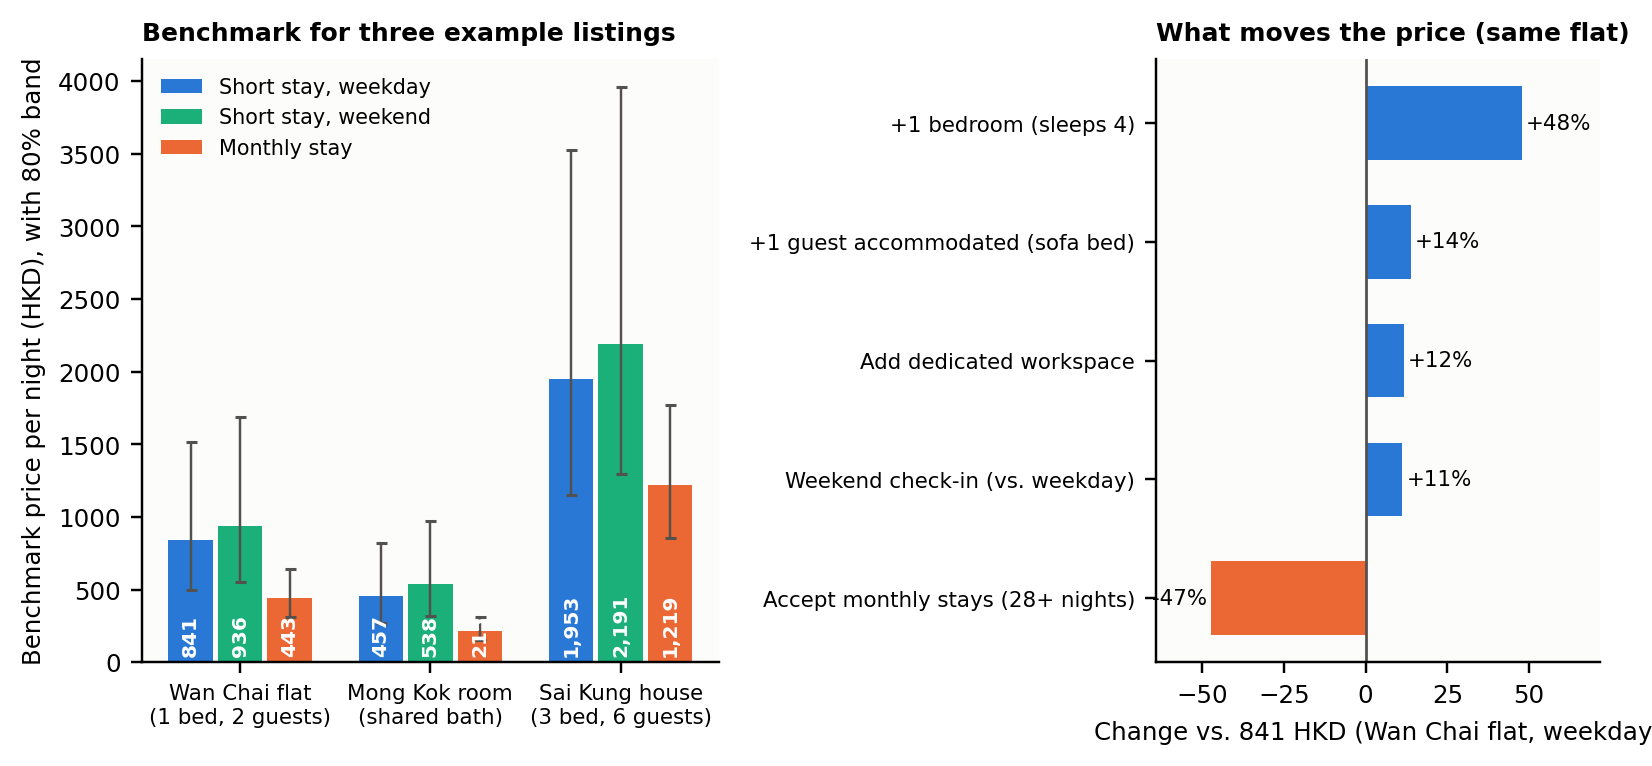
\includegraphics[width=15.2cm]{outputs/figures/fig8_decision_tool.png}\end{center}\vspace{-6pt}\nopagebreak[4]
{\fontsize{8.5}{10.2}\selectfont \color{grey} \raggedright \textbf{Figure 7 -- The decision tool.} Left: benchmark and 80\% band for three example listings under three stay types. Right: how the benchmark of one Wan Chai flat moves when a lever is changed (model-implied associations, not guaranteed returns).\par}\vspace{4pt}
{The notebook exposes the benchmark as a function: a host enters district, room and property type, guests, bedrooms, bathrooms, coordinates, stay type and amenities; the tool computes the transit and competition factors and returns a \textbf{benchmark price with an 80\% band} (from out-of-fold errors, separately for short and long stays). The band is validated: it covers 84\% of unseen listings. For a one-bedroom flat 150 m from Wan Chai station the benchmark is \textbf{841 HKD} on a weekday short stay (band 497--1,519), 936 for a weekend check-in and 443 for a monthly tenant; a shared-bathroom room in Mong Kok is 457 / 538 / 215; a three-bedroom Sai Kung house for six is 1,953 / 2,191 / 1,219. The band is wide on purpose (the 80\% band spans roughly $\times$3.1 for short stays): asking prices are noisy, and honest uncertainty is part of the product. On the lever panel, one more bedroom moves the benchmark most (+48\%), accepting monthly stays cuts the nightly price by 47\% for this flat, while individual amenities (a dedicated workspace +12\%) are small next to the band. Levers are model- and profile-dependent: the weekend premium is 12\% on average across short-stay listings in the random forest, 11\%--14\% across the three models, so we read it as 'roughly 11\%--14\%'.\par}
\begin{center}\nopagebreak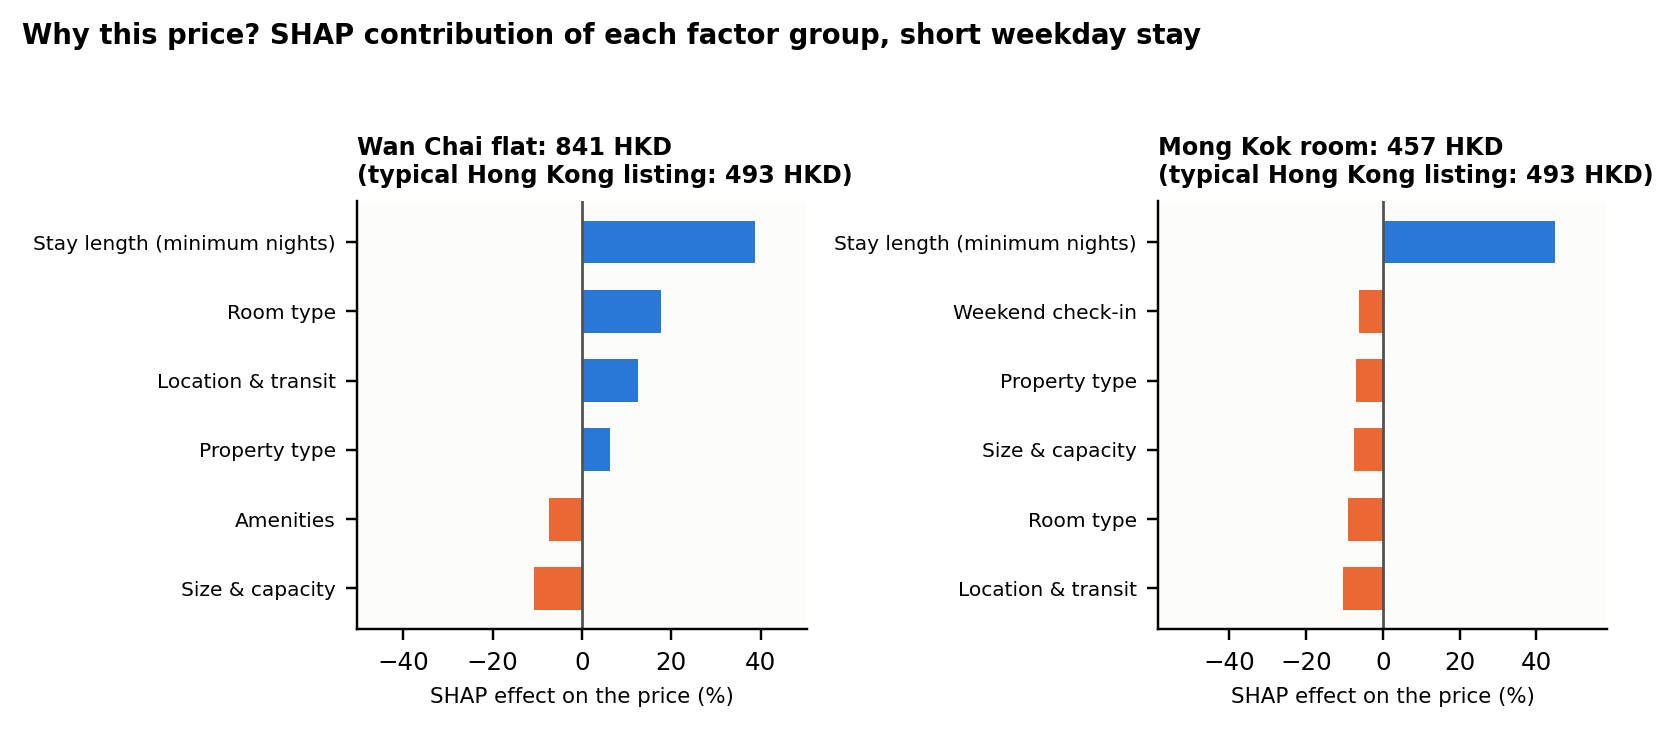
\includegraphics[width=15.2cm]{outputs/figures/fig9_explanation.png}\end{center}\vspace{-6pt}\nopagebreak[4]
{\fontsize{8.5}{10.2}\selectfont \color{grey} \raggedright \textbf{Figure 8 -- ``Why this price?'' Effect of each factor group on the benchmark, as SHAP contributions, relative to the typical Hong Kong listing (factors grouped by business meaning).}\par}\vspace{4pt}
{\textbf{Explaining each price in plain language.} A host who is told ``841 HKD'' immediately asks \textit{why}. We therefore explain every prediction with \textbf{SHAP} (Lundberg \& Lee, 2017), a standard explainability method that splits the model's prediction into one contribution per factor: starting from the typical Hong Kong listing (493 HKD), each factor pushes the price up or down and the contributions add up exactly to the prediction. We add the contributions of the factors of each business group (size, location and transit, amenities...), which gives the bars of Figure 8. A language model (OpenAI gpt-4o-mini, called through its API) then phrases these computed numbers as a short explanation; it receives only the numbers, never the data or the model. Two safeguards address the risks of AI-generated text: the factors are given to the model in two separate lists (raising and lowering the price) and a \textbf{check} rejects any number that was not supplied; a \textbf{fixed template} is used whenever the check fails or no API key is available. Output for the Wan Chai flat:\par}\vspace{-2.5pt}
{\fontsize{9}{10.8}\selectfont \color{grey} \itshape ``The benchmark price for your listing is HKD 840 per night, with an 80\% band ranging from HKD 500 to HKD 1,520. In comparison, the typical Hong Kong listing price is HKD 490. Factors associated with a higher price include a minimum stay length (39\%), room type (18\%), location and transit (13\%), and property type (6\%). Conversely, factors associated with a lower price are size and capacity (11\%) and amenities (7\%).''\par}\vspace{-0.5pt}
{\raggedright \textbf{Recommendations}\par}\vspace{-3.5pt}\nopagebreak[4]
\begin{itemize}[leftmargin=0.55cm,itemsep=2pt,topsep=2pt,parsep=0pt]
\item \textbf{Hosts and property managers.} (1) Price a new listing inside its benchmark band and move within it using what only you know (view, floor, condition). (2) Run separate weekday, weekend and monthly prices: expect a weekend premium of roughly 11\%--14\% on short stays and a monthly discount of 42\%--67\% on the median nightly price (up to 47\% for a whole flat that was priced for tourists), and decide on monthly stays by comparing the lower nightly rate with the occupancy you can sustain -- occupancy is not observable here. (3) Use the price audit (\texttt{outputs/listing\_price\_audit.csv}) as a trigger: review first any listing more than 25\% above benchmark, because that is where demand falls; for listings far below benchmark, test gradual increases, since the deepest discounts show no extra demand. (4) Spend on capacity and listing type rather than on small amenities: they dominate the model.
\item \textbf{Investors.} Choose the segment first: whole units for groups (median 1,470 HKD) and short-stay rooms behave very differently from the monthly-room segment (median 174 HKD), and professional operators dominate the latter. District matters, but transit distance is not priced separately.
\item \textbf{Platforms and policy makers.} 43\% of listings are in practice monthly rentals. Because the licence field is empty, regulators and platforms cannot see licensed versus unlicensed supply in public data; publishing it would make the market auditable.
\end{itemize}
\section*{7. Limitations and ethical considerations}
\begin{itemize}[leftmargin=0.55cm,itemsep=2pt,topsep=2pt,parsep=0pt]
\item \textbf{Asking price, one snapshot.} The price is a quote for one stay on one date, not a transaction or revenue; seasonality beyond weekend/weekday is not modelled, and listings without a price (mostly unbookable) and above the 99.5th percentile are out of scope.
\item \textbf{Association, not causation.} Premiums and the price-gap$\rightarrow$demand result are observational; unobserved quality (photos, view, floor) may drive both price and demand. Reviews are only a proxy for bookings.
\item \textbf{Data gaps and proxies.} Licence status is empty; straight-line distances ignore hills and routes; MTR data come from a volunteer map; thin districts have few listings.
\item \textbf{Explanations are model-based.} Permutation importance and SHAP values describe what the model uses, not what causes the price, and correlated factors share importance; the language-model wording is checked against the supplied numbers but remains generated text, so the template fallback exists and the explanation should be read as support, not advice.
\item \textbf{Ethics and privacy.} We use public, aggregated listing data released by Inside Airbnb; no host names, photos or reviewer identities are used or reproduced, and the audit file contains only listing ids. A price benchmark can homogenise prices if everyone follows it; it should inform, not replace, a host's judgement.
\end{itemize}
\section*{8. Conclusion}
{A machine-learning benchmark built in Python can price Hong Kong rentals 27\% more accurately than comparable-listings pricing on unseen hosts, and -- more importantly for decisions -- it explains the market: stay length and the type and size of the listing matter most; transit proximity and location details add little; and the commercial risk lies in pricing \textit{above} the benchmark, not below it. The next steps are to add transaction or occupancy data to move from asking prices to revenue, and to refresh the model periodically.\par}
\subsection*{References}
{\fontsize{8.5}{10.2}\selectfont \raggedright Breiman, L. (2001). Random forests. \textit{Machine Learning, 45}(1), 5--32.\par}\vspace{-3.5pt}
{\fontsize{8.5}{10.2}\selectfont \raggedright Hong Kong SAR Government. Hotel and Guesthouse Accommodation Ordinance (Cap. 349).\par}\vspace{-3.5pt}
{\fontsize{8.5}{10.2}\selectfont \raggedright Inside Airbnb (2026). Hong Kong listings and reviews data, scraped 25 September 2026. http://insideairbnb.com\par}\vspace{-3.5pt}
{\fontsize{8.5}{10.2}\selectfont \raggedright Lundberg, S. M., \& Lee, S.-I. (2017). A unified approach to interpreting model predictions. \textit{Advances in Neural Information Processing Systems, 30}.\par}\vspace{-3.5pt}
{\fontsize{8.5}{10.2}\selectfont \raggedright OpenStreetMap contributors. Railway station data retrieved via the Overpass API. https://www.openstreetmap.org\par}\vspace{-3.5pt}
{\fontsize{8.5}{10.2}\selectfont \raggedright Pedregosa, F., et al. (2011). Scikit-learn: Machine learning in Python. \textit{Journal of Machine Learning Research, 12}, 2825--2830.\par}\vspace{-3.5pt}
{\fontsize{8.5}{10.2}\selectfont \raggedright Rosen, S. (1974). Hedonic prices and implicit markets: Product differentiation in pure competition. \textit{Journal of Political Economy, 82}(1), 34--55.\par}\vspace{-3.5pt}
{\fontsize{8.5}{10.2}\selectfont \raggedright Xu, J. J., Chen, D., Chau, M., Li, L., \& Zheng, H. (2022). Peer-to-peer loan fraud detection: Constructing features from transaction data. \textit{MIS Quarterly, 46}(3), 1777--1792.\par}\vspace{-3.5pt}
\newpage
\section*{Appendix A -- Reproducibility and hyper-parameters}
{\fontsize{9}{10.8}\selectfont \textbf{Files.} \texttt{Code GroupName IS3240.ipynb} runs end-to-end (data in \texttt{data/}; MTR stations cached in \texttt{data/mtr\_stations.csv}; results in \texttt{outputs/}). Random seed 42; host-split seed 37. Libraries: pandas, NumPy, scikit-learn, statsmodels, shap, matplotlib, requests. The plain-language explanations use the OpenAI API when the environment variable OPENAI\_API\_KEY (or a git-ignored .env file) is set; without a key the notebook uses a deterministic template and still runs end to end.\par}
\begin{center}{\fontsize{8}{9.6}\selectfont\arrayrulecolor{rule}\begin{tabular}{>{\raggedright\arraybackslash}p{2.78cm}>{\raggedright\arraybackslash}p{11.98cm}>{\raggedleft\arraybackslash}p{1.58cm}}
\rowcolor{hdr}\color{white}\bfseries Model & \color{white}\bfseries Tuned hyper-parameters (grid search, 5-fold host-grouped CV on training data) & \color{white}\bfseries CV MAE (log)\\
Linear regression &  & 0.373\\\hline
Random forest & max\_depth=10, max\_features=0.3, min\_samples\_leaf=5 & 0.327\\\hline
Gradient boosting & learning\_rate=0.05, max\_depth=3, n\_estimators=150 & 0.323\\\hline
\end{tabular}}\end{center}
\section*{Appendix B -- Accuracy by group (test set, selected model)}
\begin{center}{\fontsize{8}{9.6}\selectfont\arrayrulecolor{rule}\begin{tabular}{>{\raggedright\arraybackslash}p{6.38cm}>{\raggedleft\arraybackslash}p{1.08cm}>{\raggedleft\arraybackslash}p{2.18cm}>{\raggedleft\arraybackslash}p{1.98cm}>{\raggedleft\arraybackslash}p{2.28cm}>{\raggedleft\arraybackslash}p{1.78cm}}
\rowcolor{hdr}\color{white}\bfseries Group & \color{white}\bfseries n & \color{white}\bfseries Median price & \color{white}\bfseries MAE (HKD) & \color{white}\bfseries Median \% error & \color{white}\bfseries Within $\pm$20\%\\
Entire home/apt | long stay & 65 & 616 & 206 & 23\% & 40\%\\\hline
Entire home/apt | short stay & 277 & 1,255 & 440 & 23\% & 44\%\\\hline
Private room | long stay & 425 & 178 & 55 & 10\% & 69\%\\\hline
Private room | short stay & 334 & 589 & 412 & 31\% & 36\%\\\hline
Private rooms, monthly & 418 & 177 & 39 & 10\% & 70\%\\\hline
Private rooms, short-stay & 293 & 580 & 388 & 29\% & 36\%\\\hline
Mixed units, short-stay, outer areas & 93 & 700 & 495 & 35\% & 30\%\\\hline
Whole units, mixed stay & 168 & 796 & 295 & 24\% & 43\%\\\hline
Whole units, short-stay, groups & 146 & 1,582 & 502 & 21\% & 45\%\\\hline
\end{tabular}}\end{center}
\section*{Appendix C -- Price map for monthly stays}
\begin{center}\nopagebreak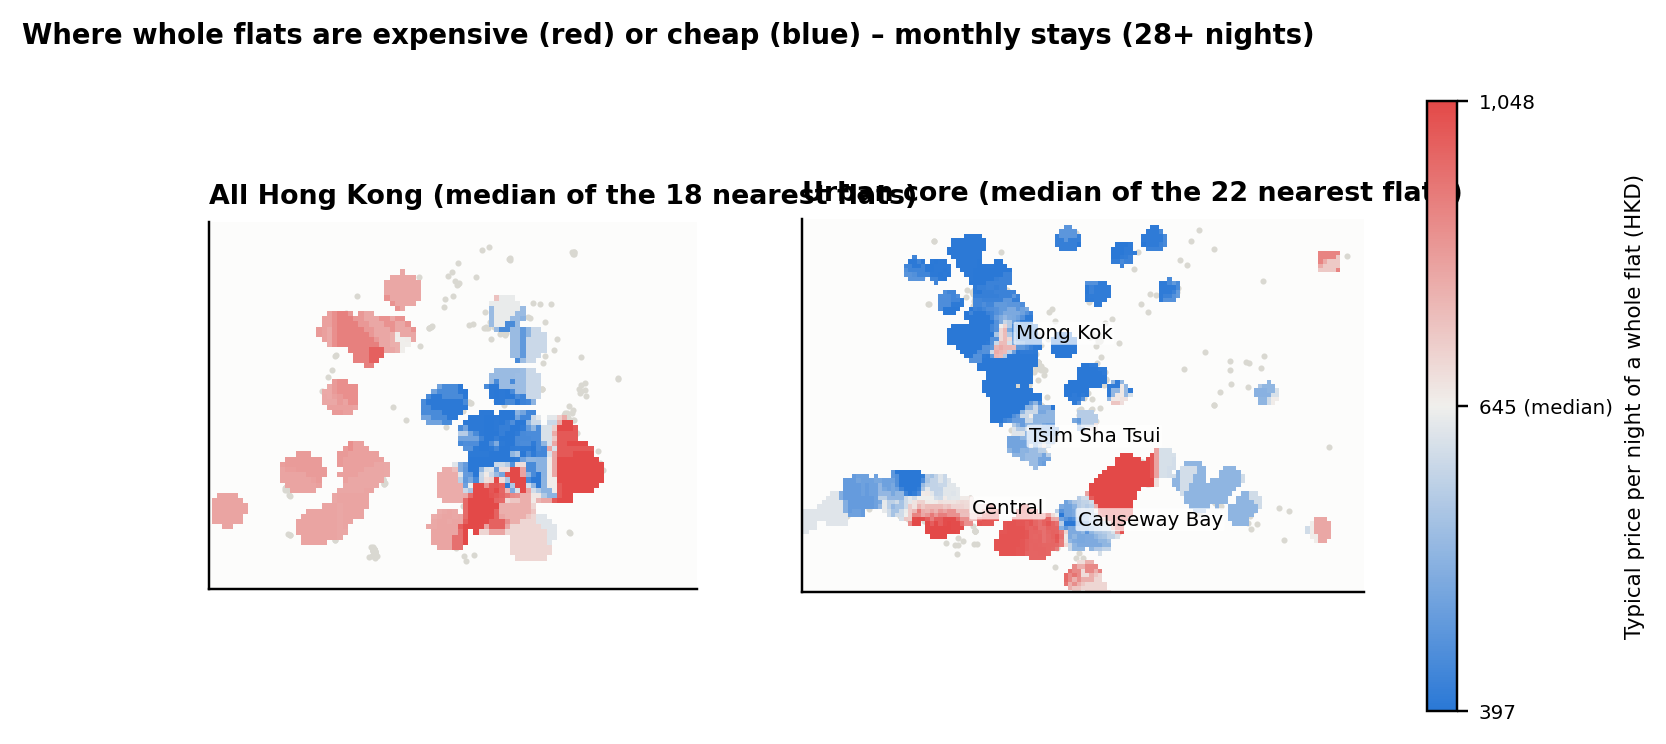
\includegraphics[width=14.6cm]{outputs/figures/fig2c_price_map_monthly.png}\end{center}\vspace{-6pt}\nopagebreak[4]
{\fontsize{8.5}{10.2}\selectfont \color{grey} \raggedright \textbf{Figure A1 -- Where whole flats are expensive (red) or cheap (blue) for monthly stays (28+ nights).}\par}\vspace{4pt}
\end{document}
